%
% A simple LaTeX template for Books
%  (c) Aleksander Morgado <aleksander@es.gnu.org>
%  Released into public domain
%

\documentclass[12pt]{book}
\usepackage[a4paper, top=3cm, bottom=3cm]{geometry}
\usepackage[utf8]{inputenc}
\usepackage[brazil]{babel}
\usepackage{graphicx}
\usepackage{subfigure}
\PassOptionsToPackage{subfigure}{tocloft}
\usepackage{setspace}
\usepackage{fancyhdr}
\usepackage{tocloft}
\usepackage{indentfirst}
\usepackage{amsmath}
\usepackage{enumitem}
\usepackage{hyperref}
\usepackage{tikz}
\usepackage{amssymb}
\usepackage{relsize}
\usetikzlibrary{shapes,arrows}
\hypersetup{
    colorlinks=true,
    linkcolor=blue,
    filecolor=magenta,      
    urlcolor=cyan,
    pdftitle={Apostila de ELE-32},
}

\addto\captionsbrazil{\renewcommand{\contentsname}{Índice}}
\let\cleardoublepage\clearpage 



\begin{document}


\pagestyle{empty}
%\pagenumbering{}
% Set book title
\title{\textbf{Apostila de ELE-32:\\Introdução a Comunicações}}
% Include Author name and Copyright holder name
\author{Prof. Manish Sharma, redigida pela COMP-18}
\date{2º Semestre de 2016}



% 1st page for the Title
%-------------------------------------------------------------------------------

\maketitle


% 2nd page, thanks message
%-------------------------------------------------------------------------------
% \thispagestyle{empty}
% \thanks{Thanks to Cicero and his \em{De finibus bonorum et malorum}}
% \newpage



% General definitions for all Chapters
%-------------------------------------------------------------------------------

% Define Page style for all chapters
\pagestyle{fancy}
% Delete the current section for header and footer
\fancyhf{}
% Set custom header
\fancyhead[RO,LE]{\thepage}
\fancyhead[LO]{\leftmark}
\fancyhead[RE]{\rightmark}
\renewcommand{\chaptermark}[1]{ \markboth{\chaptername\ \thechapter:\ #1}{} }
\renewcommand{\sectionmark}[1]{ \markright{#1}{} }

% Set arabic (1,2,3...) page numbering
\pagenumbering{arabic}

% Set double spacing for the text
%\doublespacing



% Not enumerated chapter
%-------------------------------------------------------------------------------
% \chapter*{Preface}

% Sed ut perspiciatis unde omnis iste natus error sit voluptatem accusantium
% doloremque laudantium, totam rem aperiam, eaque ipsa quae ab illo inventore
% veritatis et quasi architecto beatae vitae dicta sunt explicabo. Nemo enim
% ipsam voluptatem quia voluptas sit aspernatur aut odit aut fugit, sed quia
% consequuntur magni dolores eos qui ratione voluptatem sequi nesciunt. Neque
% porro quisquam est, qui dolorem ipsum quia dolor sit amet, consectetur,
% adipisci velit, sed quia non numquam eius modi tempora incidunt ut labore et
% dolore magnam aliquam quaerat voluptatem. Ut enim ad minima veniam, quis nostrum
% exercitationem ullam corporis suscipit laboriosam, nisi ut aliquid ex ea
% commodi consequatur? Quis autem vel eum iure reprehenderit qui in ea voluptate
% velit esse quam nihil molestiae consequatur, vel illum qui dolorem eum fugiat
% quo voluptas nulla pariatur?



% % If the chapter ends in an odd page, you may want to skip having the page
% %  number in the empty page
% \newpage
% \thispagestyle{empty}



% First enumerated chapter
%-------------------------------------------------------------------------------
% \chapter{Lorem ipsum...}

% Lorem ipsum dolor sit amet, consectetur adipiscing elit. Morbi libero sem,
% interdum eget varius vel, faucibus placerat purus. Sed vulputate diam sit amet
% risus dapibus dignissim. Praesent lobortis eleifend augue. Cum sociis natoque
% penatibus et magnis dis parturient montes, nascetur ridiculus mus. Morbi libero
% turpis, viverra ac vulputate a, faucibus vel quam. Quisque interdum congue
% lacus, in tempus nisl tincidunt at. Curabitur sed eros eu enim vehicula
% fermentum quis nec justo. Vestibulum rutrum laoreet est, eget condimentum justo
% feugiat at. Cras ac sem ac magna ornare tempor non nec nisl. Maecenas feugiat
% fringilla nisl, vitae ullamcorper ante posuere a. Sed mollis lacinia interdum.



% Last pages for ToC
%-------------------------------------------------------------------------------
% Include dots between chapter name and page number
\renewcommand{\cftchapdotsep}{\cftdotsep}
%Finally, include the ToC
{\let\cleardoublepage\clearpage
\tableofcontents
}

%-----------------------------------------------------------------------

%Semana 1
\chapter{Objetivos de um sistema de telecomunicação}

Transferir \textit{informação} de um \textit{tempo/espaço} para outro de \textit{forma eficiente}, usando os \textit{recursos disponíveis}.

\section{Informação}
Informalmente, é aquilo que não se sabe e depois se sabe. Podemos representar informações por \textit{bytes} (cadeias constituídas de sequências de 0 ou 1), e podemos medir a quantidade de informação a partir da entropia.

\section{Tempo/espaço}

\begin{center}
	\begin{figure}[!ht]
		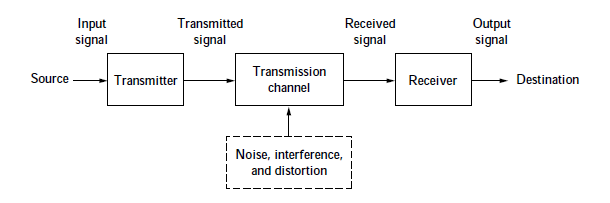
\includegraphics[scale=0.8]{figuras_cap_1/fig1.png}
        \caption{Elementos de um sistema de comunicação}
	\end{figure}
\end{center}
Os canais corrompem as mensagens de algumas maneiras:
\begin{itemize}
\item Distorção da mensagem: Perturbação do fator de forma causado por resposta imperfeita do sistema ao sinal da mensagem. Comum quando a natureza do canal é diferente da natureza da mensagem. (Exemplo: alteração no timbre da voz causada por um microfone)
\item Adição de ruído: sinais aleatórios e imprevisíveis/não-controláveis produzidos por processos naturais tanto de dentro quanto de fora do sistema (Exemplo: barulho dos carros na rua atrapalhando uma reunião dentro do prédio)
\item Interferência: contaminação por sinais externos que estejam usando o mesmo canal para se comunicar. (Exemplo: superposição de conversas próximas)
\end{itemize}

\section{Eficiência}
Garantir a transmissão de uma certa quantidade de informação com probabilidade de falha tão baixa quanto se queira.\par
Porém, há um limite máximo para sinais elétricos causado pelas duas limitações fundamentais: largura de banda e ruído. Pode-se relacionar as duas limitações pela Lei de Hartley-Shannon \footnote{Shannon, 1948}:
\begin{equation}
	R < C = B \log_2(1 + S/N)
\end{equation}
onde $R$ é a taxa de tramissão de informação, $C$ é definido como \textit{capacidade do canal}, $B$ é a largura de banda e $S/N$ é a razão de potência entre o sinal e o ruído (\textit{signal-to-noise ratio}, também chamado de SNR).

\section{Recursos disponíveis}
São, entre outros:
\begin{itemize}[nosep,label=-]
\item Potência (Energia por bit);
\item Banda disponível
\item Capacidade computacional
\item \textit{Delay} tolerável
\item Percentual de falhas tolerável
\item Número de usuários no mesmo canal
\end{itemize}

\newpage
\section*{Esquemas de sistemas de comunicação}
\begin{center}
	\begin{figure}[!ht]
		\subfigure[Broadcast]{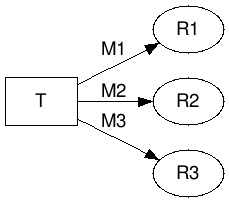
\includegraphics[width=0.3\linewidth]{figuras_cap_1/fig3.png}}
        \subfigure[Interferência]{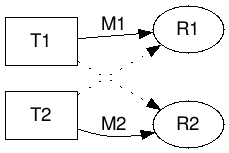
\includegraphics[width=0.3\linewidth]{figuras_cap_1/fig4.png}}
        \subfigure[Acesso Múltiplo]{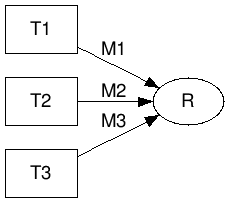
\includegraphics[width=0.3\linewidth]{figuras_cap_1/fig5.png}}
        \caption{Esquemas de transmissão dentro de um canal}
	\end{figure}
	\begin{figure}[!ht]
		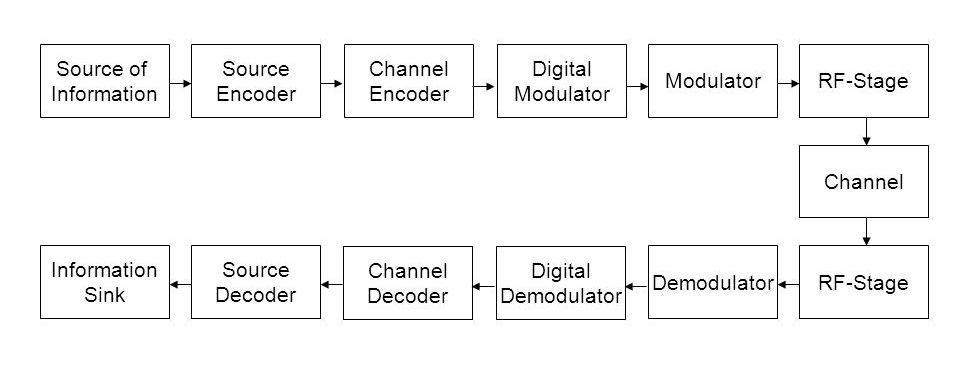
\includegraphics[scale=0.5]{figuras_cap_1/fig2.jpg}
	    \caption{Esquema de um sistema digital de comunicação}
	\end{figure}
	
\end{center}

\chapter{Densidade Espectral de potência}

\section{Correlação e autocorrelação}

%Semana 4

Dado $x(t)$ com $R_x(\tau)$ e o sistema linear invariante no tempo com resposta ao degrau $h(t)$ gerando a saída $y(t)$ com $R_y(\tau)$.

\tikzstyle{block} = [draw, fill=white!20, rectangle, 
    minimum height=3em, minimum width=6em]
\begin{center}
\begin{tikzpicture}[auto, node distance=2cm,>=latex']
    \node [block, name = x] {$x(t)$};
    \node [block, right of=x,
            node distance=3cm, name = h] {$h(t)$};
    \node [block, right of=h,
            node distance=3cm, name = y] {$y(t)$};
    \draw [->] (x) -- node[name=u] {} (h);
    \draw [->] (h) -- node[name=u] {} (y);
    \node [block, below of = x, name = Rx] {$R_x(\tau)$};
    \node [block, below of = y, name = Ry] {$R_y(\tau)$};
    \draw [<->] (x) -- node[name=u] {} (Rx);
    \draw [<->] (y) -- node[name=u] {} (Ry);
    \draw [->] (Rx) -- node[name=u] {} (Ry);
\end{tikzpicture}
\end{center}

Sabemos que $y(t) = x(t)*h(t)$.
\begin{equation}
y(t) = \int_{-\infty}^{\infty} x(\lambda) h(t-\lambda) d\lambda = \int_{-\infty}^{\infty} h(\lambda) x(t-\lambda) d\lambda
\end{equation}

\textbf{Primeiro passo:} Encontrar $R_{yx}(\tau) \triangleq \mathlarger{\int_{-\infty}^{\infty} x(t) y(t-\tau) dt}$.

\begin{equation}
R_{yx}(\tau) = \int_{-\infty}^{\infty} \bigg{[}
\int_{-\infty}^{\infty} h(\lambda)x(t-\lambda)x^*(t-\tau)d\lambda
\bigg{]}dt
\end{equation}
\begin{equation}
 = \int_{-\infty}^{\infty} h(\lambda) \bigg{[}
\int_{-\infty}^{\infty} x(t-\lambda)x^*(t-\tau)dtd\lambda
\bigg{]}
\end{equation}
\begin{equation}
 = \int_{-\infty}^{\infty} h(\lambda)
R_x(t-\lambda)d\lambda
\end{equation}

\textbf{Segundo passo:} $R_y(\tau) = \mathlarger{\int_{-\infty}^{\infty} y(t) y^*(t-\tau) dt}$
\begin{equation}
R_y(\tau) = h^*(-\tau)*R_{yx}(\tau)
\end{equation}
\begin{equation}
 = h^*(-\tau)*h(t)*R_x(\tau)
\end{equation}
\begin{equation}
 = g(\tau)*R_x(\tau)
\end{equation}

$g(\tau) = $ reposta ao impulso da autocorrelação

\section{Função de Densidade Espectral}

$x(t)$ tem densidade espectral $S_x(f)$, que informa sobre a distribuição de energia em frequência.

A densidade espectral é a transformada de Fourier da autocorrelação:

\begin{equation}
S_x(f) = \int_{-\infty}^{\infty}R_x(\tau)exp(-j 2 \pi f \tau) d\tau
\end{equation}

Como $R_x(\tau) = R_x^*(\tau)$, então $R_x(\tau)$ tem simetria hermitiana. Logo $S_x(f)$ é real.

A energia de $x(t)$ pode ser calculada como:

\begin{equation}
\label{eq: Ex por fde}
E_x = \int_{-\infty}^{\infty}S_x(f)df = TFI\{ S_x(f)\}, \tau = 0
\end{equation}
\begin{equation}
R_x(\tau) = TFI\{ S_x(f)\} = \int_{-\infty}^{\infty}S_x(f)exp(j2\pi f\tau)df
\end{equation}

Sabemos que:

\begin{equation}
R_x(\tau = 0) = \int_{-\infty}^{\infty}x(t)x^*(t)dt = E_x
\end{equation}

Logo, a equação \ref{eq: Ex por fde} é verdadeira.

\section{Relação entre sinais e sistema}

\tikzstyle{block} = [draw, fill=white!20, rectangle, 
    minimum height=3em, minimum width=6em]
\begin{center}
\begin{tikzpicture}[auto, node distance=2cm,>=latex']
    \node [block, name = x] {$x(t)$};
    \node [block, right of=x,
            node distance=3.5cm, name = h] {$h(t)$};
    \node [block, right of=h,
            node distance=4cm, name = y] {$y(t) = x(t)*h(t)$};
    \draw [->] (x) -- node[name=u] {} (h);
    \draw [->] (h) -- node[name=u] {} (y);
    \node [block, below of = x, name = X] {$X(f)$};
    \node [block, below of = y, name = Y] {$Y(f) = X(f)H(f)$};
    \node [block, below of = h, name = H] {$H(f)$};
    \draw [<->] (x) -- node[name=u] {} (X);
    \draw [<->] (y) -- node[name=u] {} (Y);
    \draw [<->] (h) -- node[name=u] {} (H);
    \draw [->] (X) -- node[name=u] {} (H);
    \draw [->] (H) -- node[name=u] {} (Y);
\end{tikzpicture}
\end{center}

\begin{equation}
x(t) \leftrightarrow R_x(\tau) \leftrightarrow S_x(f)
\end{equation}
\begin{equation}
R_{yx}(\tau) = h(\tau)*R_x(\tau)
\end{equation}
\begin{equation}
y(t) = x(t)*h(t) \leftrightarrow
R_y(\tau) = h(\tau)*h^*(-\tau)*R_x(\tau) \leftrightarrow
S_y(f) = |H(f)^2|S_x(f)
\end{equation}
\begin{equation}
g(\tau) \leftrightarrow G(f) \Rightarrow S_y(f) = G(f)S_x(f)
\end{equation}

\tikzstyle{block} = [draw, fill=white!20, rectangle, 
    minimum height=3em, minimum width=6em]
\begin{center}
\begin{tikzpicture}[auto, node distance=2cm,>=latex']
    \node [block, name = b1] {Fonte de Bits};
    \node [block, right of=b1,
            node distance=5cm, name = b2] {Codificação da fonte};
    \node [block, right of=b2,
            node distance=5.5cm, name = b3] {Codificação do canal};
    \node [block, below of=b3,
            node distance=2cm, name = b4] {Modulação digital};
    \node [block, below of=b4,
            node distance=2cm, name = b5] {Modulador};
    \node [block, left of=b5,
            node distance=5.5cm, name = b6] {Canal};
    \node [block, left of=b6,
            node distance=5cm, name = b7] {Demodulador};
    \node [block, below of=b7,
            node distance=2cm, name = b8] {Demodulação digital};
    \node [block, right of=b8,
            node distance=5cm, name = b9] {Decodificação de canal};
    \draw [->] (b1) -- node[name=u] {} (b2);
    \draw [->] (b2) -- node[name=u] {} (b3);
    \draw [->] (b3) -- node[name=u] {} (b4);
    \draw [->] (b4) -- node[name=u] {} (b5);
    \draw [->] (b5) -- node[name=u] {} (b6);
    \draw [->] (b6) -- node[name=u] {} (b7);
    \draw [->] (b7) -- node[name=u] {} (b8);
    \draw [->] (b8) -- node[name=u] {} (b9);
    \draw [color=gray,thick](-2,-5) rectangle (12,-3);
	\node at (-0.5,-3) [above=5mm, right=0mm] {\textsc{Canal vetorial}};
\end{tikzpicture}
\end{center}

%Item 9 - Murilo

\chapter{Sinais e sistemas em banda base e banda passante}

\section{Equivalência}

Sinal em \underline{banda base} tem conteúdo em torno de $f=0$.

\underline{Banda do sinal menor}: valor de W tal que \( |X(f)|=0\) p/ \(|f|>W \)

Bandas de x\% de energia

\underline{Banda de 3dB}: \( W_{3dB} \) tal que \( |X(f)|< \frac{max[\,X(f)]\,}{2} \)  p/ \( |f| > W_{3dB} \).

Sinal em \underline{Banda Passante}: tem conteúdo em torno de $f_c$ (frequência central).

Banda do sinal $W=f_2 - f_1$ tal que p/ $f>0$, $|X(f)|=0$ p/ $f>f_2$ ou $f<f_1$.

\section{Conversão de Banda Base para Banda Passante}

Sinais reais tem simetria Hermitiana, logo um dos lados do espectro contém toda a informação necessária sobre o sinal.

Definimos: 
\begin{equation}
X_+ (f)=2.u(f).X(f)
\end{equation}
\begin{equation}
x_+ (t) = x(t)*\{2.\mathcal{F}^{-1}\{u(f)\}\} = x(t)*[\, 2(\, \frac{1}{j2\pi t} + \frac{\delta (t)}{2} )\, ]\,
= x(t)*[\, \delta (t) - \frac{1}{j \pi t} ]\, = 
\end{equation}








\end{document}

